\documentclass{anstrans}
%%%%%%%%%%%%%%%%%%%%%%%%%%%%%%%%%%%
\title{Application of the entropy viscosity method to the 1-D 7-equation Model for Two-Phase Flows}
\author{Marc O. Delchini$^{*}$, Jean C. Ragusa$^{*}$, Ray A. Berry$^\dagger$}

\institute{
$^{*}$Department of Nuclear Engineering, Texas A\&M University, 
$^\dagger$Idaho National Laboratory
}

\email{delcmo@tamu.edu \and jean.ragusa@.tamu.edu \and ray.berry@inl.gov}

% Optional disclaimer: remove this command to hide
%\disclaimer{Notice: This manuscript is a work of fiction. Any resemblance to actual articles, living or dead, is purely coincidental.}

%%%% packages and definitions (optional)
\usepackage{graphicx} % allows inclusion of graphics
\usepackage{booktabs} % nice rules (thick lines) for tables
\usepackage{microtype} % improves typography for PDF
%\usepackage{subfigure}
\usepackage{subcaption}
\usepackage{float}
\setlength{\columnsep}{0.5 in}

\renewcommand{\div}{\vec{\nabla}\! \cdot \!}
\newcommand{\grad}{\vec{\nabla}}
\newcommand{\divv}[1]{\vec{\nabla}^{#1}\! \cdot \!}
\newcommand{\gradd}[1]{\vec{\nabla}^{#1}}
% latex shortcuts
\newcommand{\bea}{\begin{eqnarray}}
\newcommand{\eea}{\end{eqnarray}}
\newcommand{\be}{\begin{equation}}
\newcommand{\ee}{\end{equation}}
\newcommand{\bal}{\begin{align}}
\newcommand{\eali}{\end{align}}
\newcommand{\bi}{\begin{itemize}}
\newcommand{\ei}{\end{itemize}}
\newcommand{\ben}{\begin{enumerate}}
\newcommand{\een}{\end{enumerate}}
% DGFEM commands
\newcommand{\jmp}[1]{[\![#1]\!]}                     % jump
\newcommand{\mvl}[1]{\{\!\!\{#1\}\!\!\}}             % mean value
\newcommand{\keff}{\ensuremath{k_{\textit{eff}}}\xspace}
% shortcut for domain notation
\newcommand{\D}{\mathcal{D}}
% vector shortcuts
\newcommand{\vo}{\vec{\Omega}}
\newcommand{\vr}{x}
\newcommand{\vn}{\vec{n}}
\newcommand{\vnk}{\vec{\mathbf{n}}}
\newcommand{\vj}{\vec{J}}
\newcommand{\eig}[1]{\| #1 \|_2}

\newcommand{\EI}{\mathcal{E}_h^i}
\newcommand{\ED}{\mathcal{E}_h^{\partial \D^d}}
\newcommand{\EN}{\mathcal{E}_h^{\partial \D^n}}
\newcommand{\ER}{\mathcal{E}_h^{\partial \D^r}}
\newcommand{\reg}{\textit{reg}}

\newcommand{\norm}{\textrm{norm}}
\renewcommand{\Re}{\textrm{Re}}
\newcommand{\Pe}{\textrm{P\'e}}
\renewcommand{\Pr}{\textrm{Pr}}

\newcommand{\resi}{R}
%\newcommand{\resinew}{\tilde{D}_e}
\newcommand{\resinew}{\widetilde{\resi}}
\newcommand{\matder}[1]{\frac{\textrm{D} #1}{\textrm{D} t}}


% extra space
\newcommand{\qq}{\quad\quad}
% common reference commands
\newcommand{\eqt}[1]{Eq.~(\ref{#1})}                     % equation
\newcommand{\fig}[1]{Fig.~\ref{#1}}                      % figure
\newcommand{\tbl}[1]{Table~\ref{#1}}                     % table
\newcommand{\sct}[1]{Section~\ref{#1}}                   % section
\newcommand{\app}[1]{Appendix~\ref{#1}}                   % appendix

\newcommand\br{\mathbf{r}}
%\newcommand{\tf}{\varphi}
\newcommand{\tf}{b}


\begin{document}
%%%%%%%%%%%%%%%%%%%%%%%%%%%%%%%%%%%%%%%%%%%%%%%%%%%%%%%%%%%%%%%%%%%%%%%%%%%%%%%%
\section{Introduction}
%
In this paper, we extend the entropy viscosity method, proposed by Guermond et al. \cite{jlg1, jlg2}
to the well-posed 1-D 7-equation two-phase model \cite{DEM, berry}. This model is obtained by integrating the single-phase flow balance equations weighed by a characteristic function for each phase. The resulting system of equations contains non-conservative terms that describe the interaction between phases but also an equation for the volume fraction. This two-phase flow model is also known to be unconditionally hyperbolic, which is highly desirable when working with approximate Riemann solvers, and can be used for a wide range of applications. Its particularity comes from the pressure and velocity relaxation terms appearing in the volume fraction, momentum, and energy equations. When employing large values for the relaxation parameters, the two phases come be brought in equilibrium. The 7-equation model can degenerate into the 6-equation model (same phasic pressure) \cite{Toumi_1996} and the 5-equation model (same phasic velocities and pressure) \cite{Kapila_2001}. The 7-equation model is currently discretized in space using \emph{discontinuous schemes} with approximate Riemann solvers derived from the well-established approaches for single-phase flows, while using an upwind-type flux for the non-conservative terms \cite{Saurel_2001a, Saurel_2001b, Li_2004, Zein_2010, Ambroso_2012}. 

% Here, we propose to to discretized the system of equations using a continuous finite element method, 
% stabilized using the entropy viscosity technique.
The entropy viscosity technique is a viscous regularization technique
that satisfies the entropy minimum principle; adequate dissipation terms (viscous fluxes)
are added to the governing laws while ensuring the entropy minimum principle still holds.
Viscosity coefficients modulates the magnitude of the added dissipation such that it is
large in shock regions and vanishingly small elsewhere. The entropy viscosity coefficients
are taken proportional to the entropy production while, at the same time, being bounded
from above by a first-order viscosity coefficient that reduces the spatial discretization
to be similar to a first-order Godunov scheme (the latter being known to be overly dissipative but
monotone \cite{toro}). Hence, entropy production in shocks will result in large viscosity  
coefficients and thus will avoid spurious oscillations. 

The entropy method is independent of the type of spatial discretization (finite volume,
continuous or discontinuous finite elements, ...) and thus can be applied ubiquitously. 
The results presented in this summary were obtained with RELAP-7 \cite{Berry_2014}, the next-generation 
reactor safety system code built upon the MOOSE multiphysics framework
\cite{moose} that uses a \emph{Continuous Galerkin Finite Element Method}.

In this summary, the 1-D 7-equation model is recalled along with the dissipative terms used 
in the entropy method. Definition of the viscosity coefficients is also given and numerical 
results are presented for a 1-D two-phase flow shock tube.
%
%%%%%%%%%%%%%%%%%%%%%%%%%%%%%%%%%%%%%%%%%%%%%%%%%%%%%%%%%%%%%%%%%%%%%%%%%%%%%%%%
\section{Theory}
%
We recall the 1-D 7-equation model for phase $k$ in interaction with phase $j$ where we have already added, for conciseness, the viscous regularization
terms based on the entropy-viscosity method: % (equation of the phase $j$ are obtained by simply substituting $k$ by $j$):
\begin{subequations}
\label{eq:euler_visc}
%
\begin{equation}\label{eq:vf_eq}
  \frac{\partial \alpha_{k} A}{\partial t} + u_{int} A \frac{\partial \alpha_{k}}{\partial x}
  = A \mu_P (p_{k} - p_{j}) + \boxed{\frac{\partial }{\partial x} \left( A l_k  \right)}
\end{equation}
%
\begin{eqnarray}
  \frac{\partial \left( \alpha \rho \right)_{k} A}{\partial t}
  + \frac{\partial \left( \alpha \rho u \right)_{k} A}{\partial x}
  = \boxed{\frac{\partial }{\partial x} \left( A f_k \right)}
\end{eqnarray}
%
\begin{eqnarray}
 && \frac{\partial \left( \alpha \rho u \right)_{k} A}{\partial t}
  + \frac{\partial \alpha_{k} A \left( \rho u^2 + p \right)_{k} }{\partial x}   = p_{int} A \frac{\partial \alpha_{k}}{\partial x} \nonumber \\
 &&+ p_{k} \alpha_{k} \frac{\partial A}{\partial x}
  + A \lambda_u (u_{j} - u_{k}) \nonumber \\
 && + \boxed{\frac{\partial }{\partial x} \left[ A \left( g_k + u_k f_k \right) \right] }
\end{eqnarray}
%
\begin{eqnarray}
 &&\frac{\partial \left( \alpha \rho E \right)_{k} A}{\partial t}
  + \frac{\partial \alpha_{k} u_{k} A \left( \rho E + p \right)_{k}}{\partial x}
  = p_{int} u_{int} A \frac{\partial \alpha_{k}}{\partial x} 
  \nonumber \\
  &&- \bar{p}_{int} A \mu_P (p_{k} - p_{j})+ \bar{u}_{int} A \lambda_u (u_{j} - u_{k})
  \nonumber \\
 && + \boxed{\frac{\partial }{\partial x} \left[ A \left( h_k + u_k g_k - \frac{u_k^2}{2}f_k + \rho_k e_k l_k\right) \right] }
\end{eqnarray}
%
\end{subequations}
where the dissipative terms, boxed in Eq~.\ref{eq:euler_visc}, have the following definition:
\begin{subequations}
%
\begin{equation}
  l_k = \beta_k \partial_x \alpha_k 
\end{equation}
%  
\begin{equation}
  f_k = \alpha_k \kappa_k \partial_x \rho_k + \rho_k l_k 
\end{equation}
%  
\begin{equation}
  g_k = \alpha_k \mu_k \rho_k \partial_x u_k 
\end{equation}  
%
\begin{equation}
  h_k =  \alpha_k \kappa_k \partial_x \left( \rho_k e_k \right)
 \end{equation}
%
\end{subequations}
The notation is standard: $\alpha_k$, $\rho_k$, $(\rho \vec{u})_k$ and $(\rho E)_k$ are the volume fraction, the density, the momentum and the total energy for phase $k$, respectively, and will be referred to as the conservative variables. $u_k$ is the fluid velocity for phase $k$ and its specific internal energy is denoted by $e_k=E_k-\tfrac{u^2_k}{2}$. The area $A$ is a given and can be spatial-dependent. An equation of state is used to compute the pressure $P_k$. Definitions of the interfacial variables denoted by the subscript $int$ can be found in \cite{berry}. As mentioned in the introduction, each viscosity coefficient is function of an upper bound refer to as the first-order viscosity and denoted by the subscript max, and a high-order viscosity coefficient denoted by the subscript $e$ as follows: 
%
\begin{align}
&\mu_k^K(x_q,t) = \min ( \mu_{max,k}^K(x_q,t), \mu_{e,k}^K(x_q,t) ) \text{, } \nonumber \\
&\kappa_k^K(x_q,t) = \min ( \kappa_{max,k}^K(x_q,t), \kappa_{e,k}^K(x_q,t) )\nonumber  \\ 
\text{ and } &\beta_k^K(x_q,t) = \min ( \beta_{max,k}^K(x_q,t), \beta_{e,k}^K(x_q,t) ) \nonumber
\end{align}
%
where $K$ is a given element of the mesh, and $x_q$ is a quadrature point location within cell $K$.
The first-order viscosity coefficients, $\mu^K_{max,k}$ and $\kappa^K_{max,k}$, are only present in the continuity, momentum and energy equations of each phase, and thus are defined proportional to the local maximum eigenvalue $u_k + c_k$. 
%
\begin{align}
&\kappa_{max,k}^K(x_q,t) = \mu_{max,k}^K(x_q,t) = \frac{h^k}{2} (u_k(x_q,t) || +c_k(x_q,t) ) \nonumber \\
&\beta_{max,k}^K(x_q,t) = \frac{h^K}{2} ||u_{int}(x_q,t) ||, \nonumber
\end{align}
%
where $h^K$ is the grid size of element $K$. On the other hand, the first-order viscosity coefficient $\beta^K_{max,k}$ is defined proportional to the eigenvalue $u_{int}$ since intimately related to the void fraction equation. The high-order viscosity coefficients, $\beta^K_{e,k}$, $\kappa^K_{e,k}$ and $\mu^K_{e,k}$ are distinct positive viscosity coefficients and are based on the local entropy production in phase $k$. The definition of the coefficients $\mu^K_{e,k}$ and $\kappa^K_{e,k}$ is identical to the one used for the multi-D Euler equations \cite{marco_inl_report} and yield well-scaled dissipative terms in the low-Mach regime \cite{LowMach1, LowMach2, LowMach3}:
%
\begin{subequations}
\label{eq:ent_visc_coeff2}
\begin{equation}
\kappa^K_{e,k}(x_q,t) =  h_K^2 \frac{\max \left( | \resinew_k^K(x_q,t) |, J_P^K \right)}{\rho_k c_k^2}  
\end{equation}
\begin{equation}
\mu^K_{e,k}(x_q,t) = Pr_k \, \kappa^K_e(x_q,t)
\end{equation}
\end{subequations}
%
where $c_k$ is the phase speed of sound and the weighting factor is the local Mach number, $M_k=u_k/c_k$. $\Pr_k$ is the Prandtl number; see \cite{jlg1} for additional details. The entropy residual is denoted by $\resinew$ and its definition is recalled in \eqt{eq:ent2_res}.  
%
\begin{equation}
\label{eq:ent2_res}
\resinew(\vec{r_q},t) := \left( \matder{P_k} - c^2_k \matder{\rho_k} \right) , %\propto \partial_t s_k + \vec{u} \cdot \grad s_k = \matder{s_k},
\end{equation} 
%
where $s_k$ is the phase entropy, function of the density $\rho_k$ and the internal energy $e_k$. Proof of \eqt{eq:ent2_res} can be found in \cite{marco_inl_report}. Lastly, the quantity $J_P$ denotes the inter element jumps of the gradient of the pressure and the density (see \cite{marco_inl_report} for details).

The approach to define the viscosity coefficient $\beta_{e,k}^K$ is similar to the logic followed for hyperbolic scalar equations \cite{jlg1, jlg2}: an entropy equation can be derived from the volume fraction equation (\eqt{eq:vf_eq}) and used in the definition of the coefficient $\beta_{e,k}^K$. Following the work by Guermond et al. \cite{jlg1, jlg2}, one obtains:
%
\begin{subequations}
\begin{equation}
\beta^K_{e,k}(x_q,t) =  h_K^2 \frac{\max \left( | R_{\alpha,k}^K(x_q,t) |, J^K_\alpha \right)}{\alpha_k},
\end{equation}
where the entropy residual associated to the volume fraction equation, \eqt{eq:vf_eq}, is
\begin{equation}
\label{eq:beta_def}
R_{\alpha,k}^K(x_q,t) =   \frac{1}{2} \left( \frac{\partial \alpha_{k}^2}{\partial t} + u_{int} \frac{\partial \alpha_{k}^2}{\partial x} \right).
\end{equation} 
\end{subequations}
% 
amd $J^K_\alpha$ denotes the inter element jump of the gradient of the volume fraction.
%where $s_{\alpha,k} = \alpha_k^2/2$ can be interpreted as the entropy function associated to the volume fraction equation of phase $k$. Once again, $J^K_\alpha$ %denotes the inter element jump of the gradient of the volume fraction.

%%%%%%%%%%%%%%%%%%%%%%%%%%%%%%%%%%%%%%%%%%%%%%%%%%%%%%%%%%%%%%%%%%%%%%%%%%%%%%%%
\section{Results and Analysis}

The 1-D 7-equation model with viscous stabilization is discretized with {\it continuous} finite elements in space and BDF2 in time using RELAP-7. The resulting nonlinear system of equations at each time step is solved using a Jacobian-free Newton Krylov technique. We present one sample result for a 1-D two-phase flow shock tube of length $L=1$ $m$ and area $A=1$ $m^2$ filled with two gas phases in equilibrium (same pressure and velocity) described by the ideal gas equation of state with $\gamma_1 = 3$ and $\gamma_2 = 1.4$, with the objective of testing adequacy of our numerical stabilization method. Initially, a membrane separates the shock tube pipe in two chambers, one with a high pressure ($P_{left} = 1$ $MPa$) on the left side and another one with a low pressure ($P_{right} = 0.1$ $MPa$) on the right. Both phases are initially at rest. The volume fraction is set to 0.5 which means each side of the chamber contains a mixture of two phases with different equation of state parameters. The pressure and velocity relaxation coefficients are computed using the expression provided in \eqt{E-R:85}. 
%
\begin{equation}\label{E-R:85}
  \lambda_u = \frac{1}{2} \mu_P Z_{1} Z_{2} \text{ and }
  \mu_P = \frac{A_{int}}{Z_{1}+Z_{2}} 
\end{equation}
%
where the interfacial area is set to a large value, $A_{int} = 10^4 m^{-1}$, so that the two phases achieve pressure and velocity equilibrium at all time. The geometry is discretized with an uniform mesh of 500 cells and the simulation is run with a CFL of 1 until $t_{final} = 305$ $\mu s$. The numerical results are presented in\fig{fig:pressure} to \ref{fig:viscosity_coeff_beta}. An exact solution for this shock tube test is not available but numerical results obtained with a discontinuous scheme on a moving mesh can be found in \cite{Saurel_2007} and use for comparison.\\

As expected, the two fluids have the same pressure and velocity profiles as shown in \fig{fig:pressure} and \fig{fig:velocity}, respectively. The shock is well resolved and does not display any instability. The density of phases 1 and 2 have different values but experience similar variations (shock, contact and rarefaction waves), as shown in \fig{fig:density}. The volume fraction varies because of the pressure relaxation term (\eqt{eq:vf_eq}) and displays a shock wave around $x=0.7$ $m$ as shown in \fig{fig:volume_fraction}. Consequently, the viscosity coefficient $\beta_k$ is peaked in the shock region and also displays a second peak of lower amplitude at the location of the contact wave. \fig{fig:viscosity_coeff_vap} and \fig{fig:viscosity_coeff_liq} show the viscosity coefficients $\mu_k$ and $\kappa_k$ for phase $1$ and $2$, respectively: they are peaked in the shock region and also display a smaller peak in the contact wave. Overall, the numerical solution is efficiently stabilized by the entropy viscosity method and the discontinuities are well resolved. %The viscosity coefficients are peaked in the shock region and thus, behave as expected. 

%The same 1-D shock tube could be run when setting the relaxation coefficients to zero: the two fluids would behave independently of each other and the volume fraction would remain constant. This test is 
%of area $A = 10^{-4}$ $m^2$ with a wall heat source (the wall temperature is constant: $T_w = 550$ $K$). The stiffened gas equation of state is used to model the liquid and vapor phases with the parameters taken from \cite{SGEOS} for each phase. A static pressure of $P=7.1$ $MPa$ is set at the outlet. The volume fraction, the enthalpy and the mass flow rate are specified at the inlet for each phase. The wall friction coefficient is constant and the same for the two phases, $f_w = 4 \times 10^{-2}$. The interfacial area $A_{int}$ is set to a large value to equalize the pressure and velocity of the two phases (the 7-equation model degenerates in to the 5-equation model). The initial conditions are uniform. The geometry is discretized with a uniform mesh of 100 elements and the simulation is run with $CFL=100$  until a steady state is obtained. 
%
%The pressure, temperature, velocity, volume fraction and viscosity coefficients profiles are plotted from \fig{fig:pressure} through \fig{fig:viscosity_coeff}. As expected, the liquid and vapor pressure profiles are identical (\fig{fig:pressure}) and decrease through the domain because of the wall friction force. The liquid and velocity profiles are also identical as shown in \fig{fig:velocity} and increase due to the wall friction force and the heat addition. In \fig{fig:temperature}, the liquid and vapor temperature profiles are distinct and have  the same variation: the temperature rises since energy is added to the flow by the wall heat source. The variations of the vapor and liquid volume fractions are opposite: vapor is produced since the liquid temperature is larger than the saturation temperature. All of the profiles are smooth and do not display any spurious oscillations: the high-order viscosity coefficients shown in \fig{fig:viscosity_coeff}, $\kappa_{e,k}$ and $\beta_{e,k}$, are well-scaled and large enough to stabilize the numerical solution without altering it (only $\beta_{e,liquid}$ is plotted since $\beta_{e,liquid}=\beta_{e,vapor}$). It is also noted the difference of several order of magnitude between the high-order and first-order viscosity coefficients denoted by the subscript $max$. The first-order viscosity coefficients are over-dissipative and ill-scaled in the low Mach regime \cite{marco_inl_report}.
%
%%%%%%%%%%%%%%%%%%%%%%%%%%%%%%%%%%%%%%%%%%%%%%%%%%%%%%%%%%%%%%%%%%%%%%%%%%%%%%%%
\section{Conclusions}

We have presented an extension of the entropy viscosity method to the 1-D 7-equation two-phase model and applied it to a shock tube problem with large relaxation coefficients. The numerical results show that the stabilization method is capable of stabilizing the schemes and that the viscosity coefficients are well-scaled. This work will further contribute to the assessment of the stabilization technique for reactor flow problems in RELAP-7.

%%%%%%%%%%%%%%%%%%%%%%%%%%%%%%%%%%%%%%%%%%%%%%%%%%%%%%%%%%%%%%%%%%%%%%%%%%%%%%%%

\begin{figure}[H]
        \centering
        %\begin{subfigure}[b]{0.5\textwidth}
                %\centering
                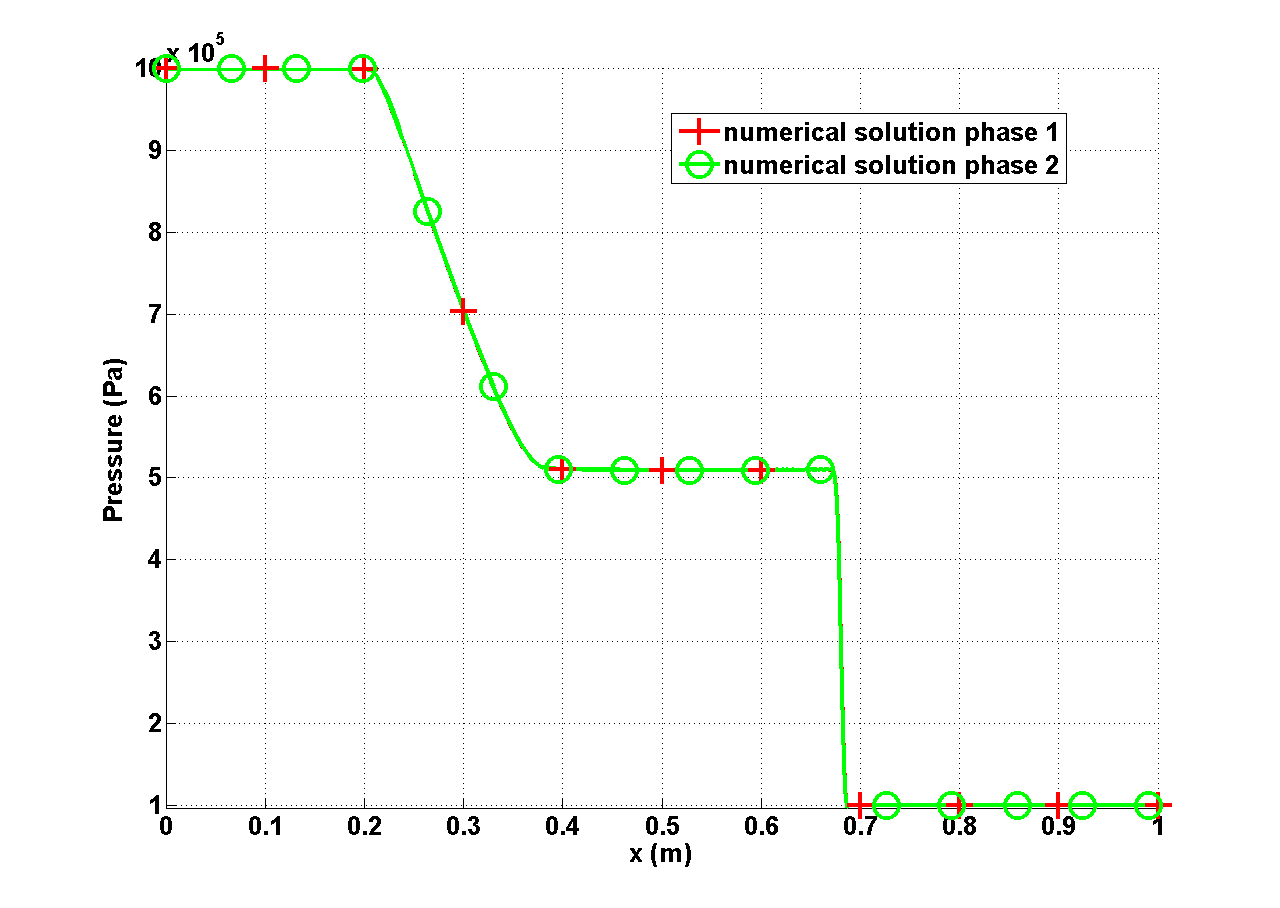
\includegraphics[width=0.495\textwidth]{plots/relaxation_two_phases_pressure.png}
                \caption{Pressure at steady state.}
                \label{fig:pressure}
        %\end{subfigure}%
\end{figure}
\begin{figure}[H]

        %\begin{subfigure}[b]{0.5\textwidth}
                %\centering
                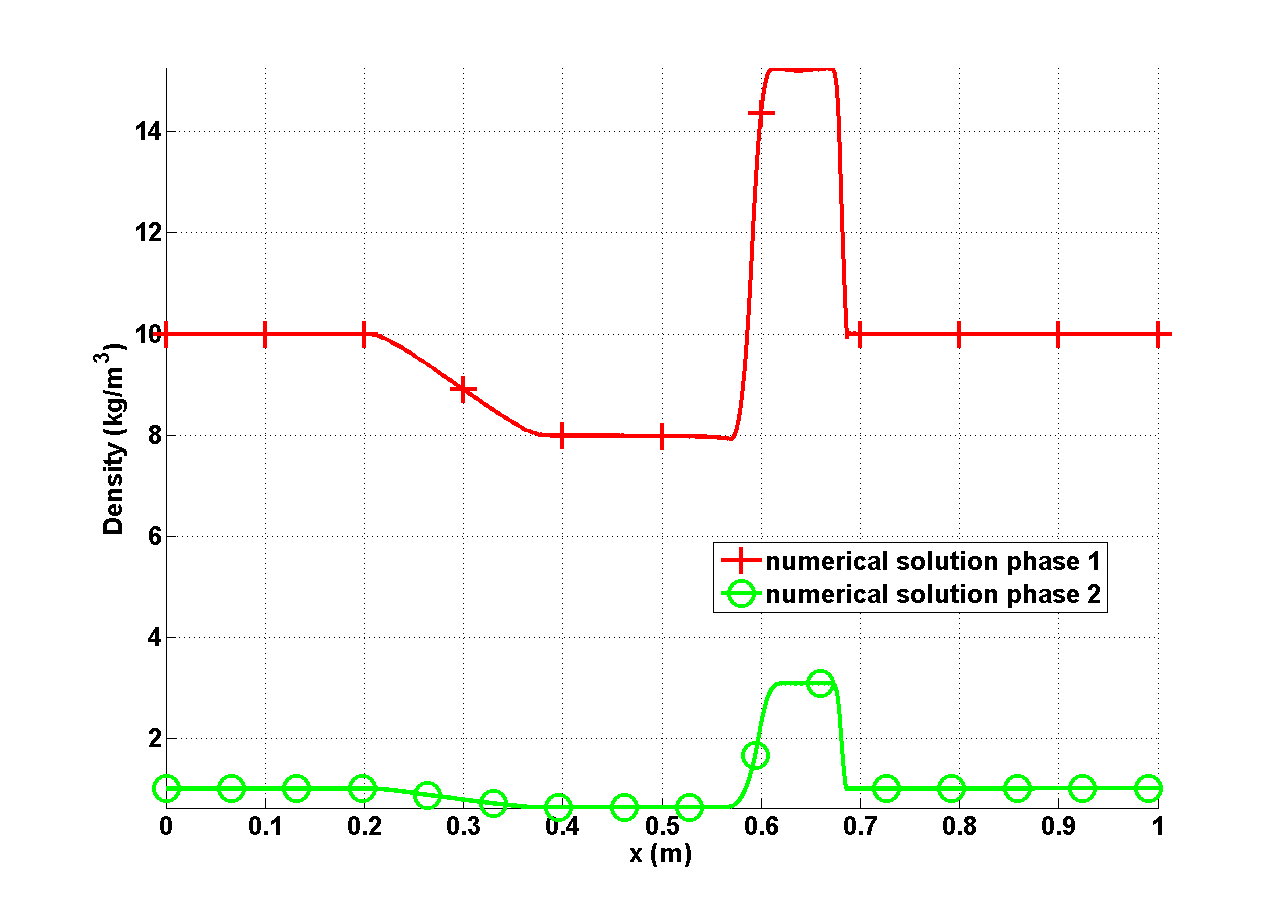
\includegraphics[width=0.495\textwidth]{plots/relaxation_two_phases_density.png}
                \caption{Density at steady state.}
                \label{fig:density}
        %\end{subfigure}%
\end{figure}
\begin{figure}[H]
        %\begin{subfigure}[b]{0.495\textwidth}
                \centering
                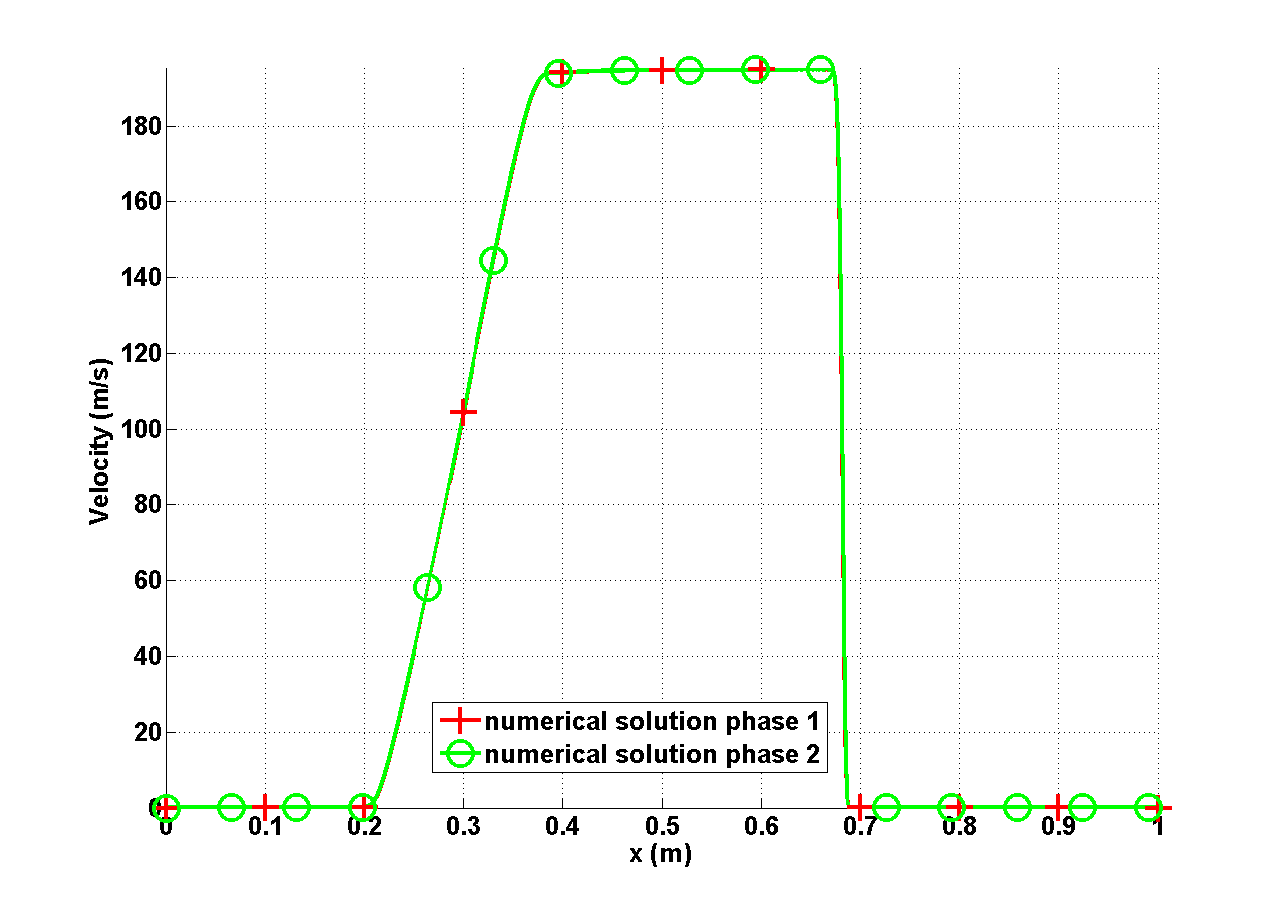
\includegraphics[width=0.495\textwidth]{plots/relaxation_two_phases_velocity.png}
                \caption{Velocity at steady state.}
                \label{fig:velocity}
        %\end{subfigure}
\end{figure}
\begin{figure}[H]
        %\begin{subfigure}[b]{0.495\textwidth}
                \centering
                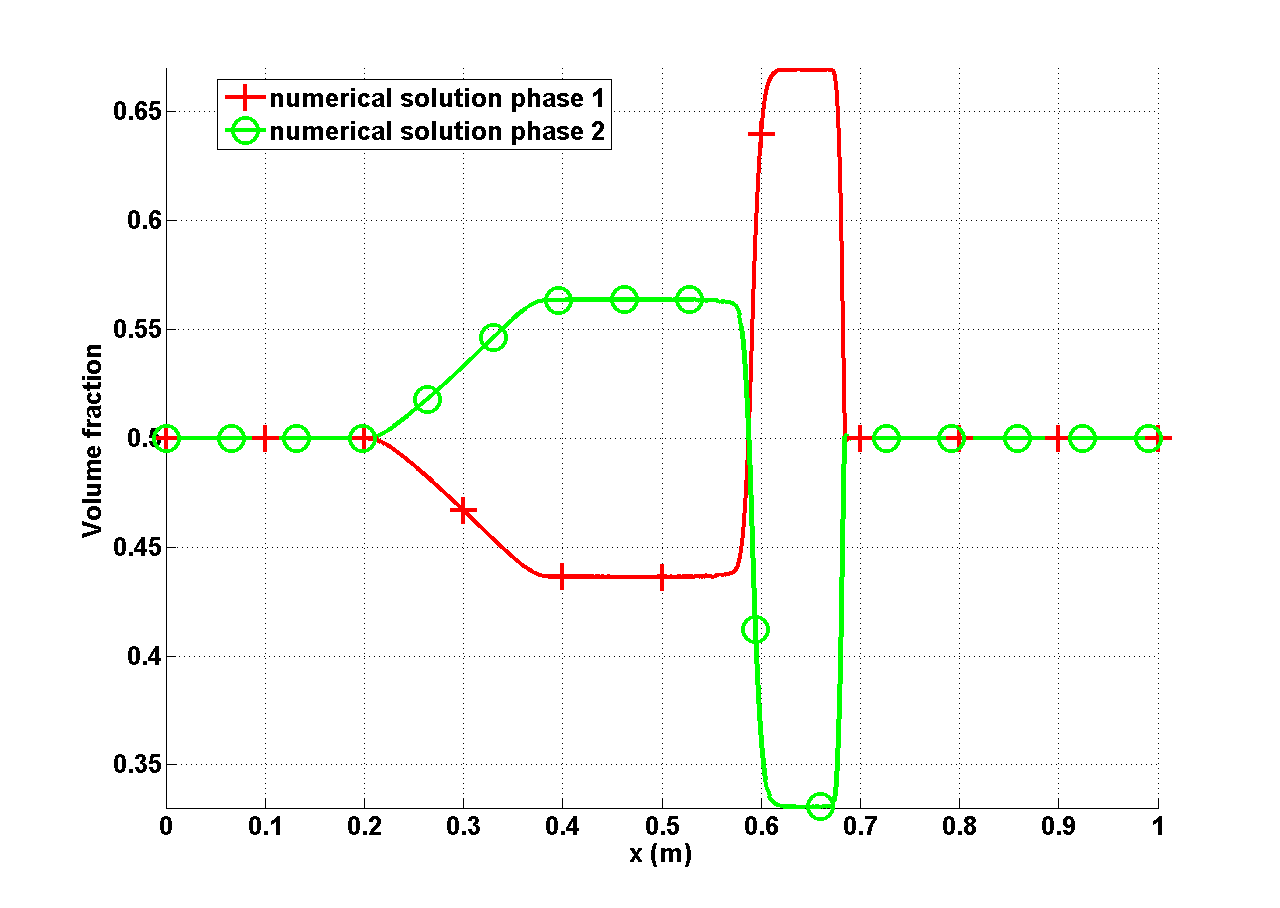
\includegraphics[width=0.495\textwidth]{plots/relaxation_two_phases_volume_fraction.png}
                \caption{Volume fraction at steady state.}
                \label{fig:volume_fraction}
        %\end{subfigure}
				%\caption{Pressure, density, velocity and void fraction at steady state.}
\end{figure}
\begin{figure}[H]    
%        \begin{subfigure}[b]{0.495\textwidth}
                \centering
                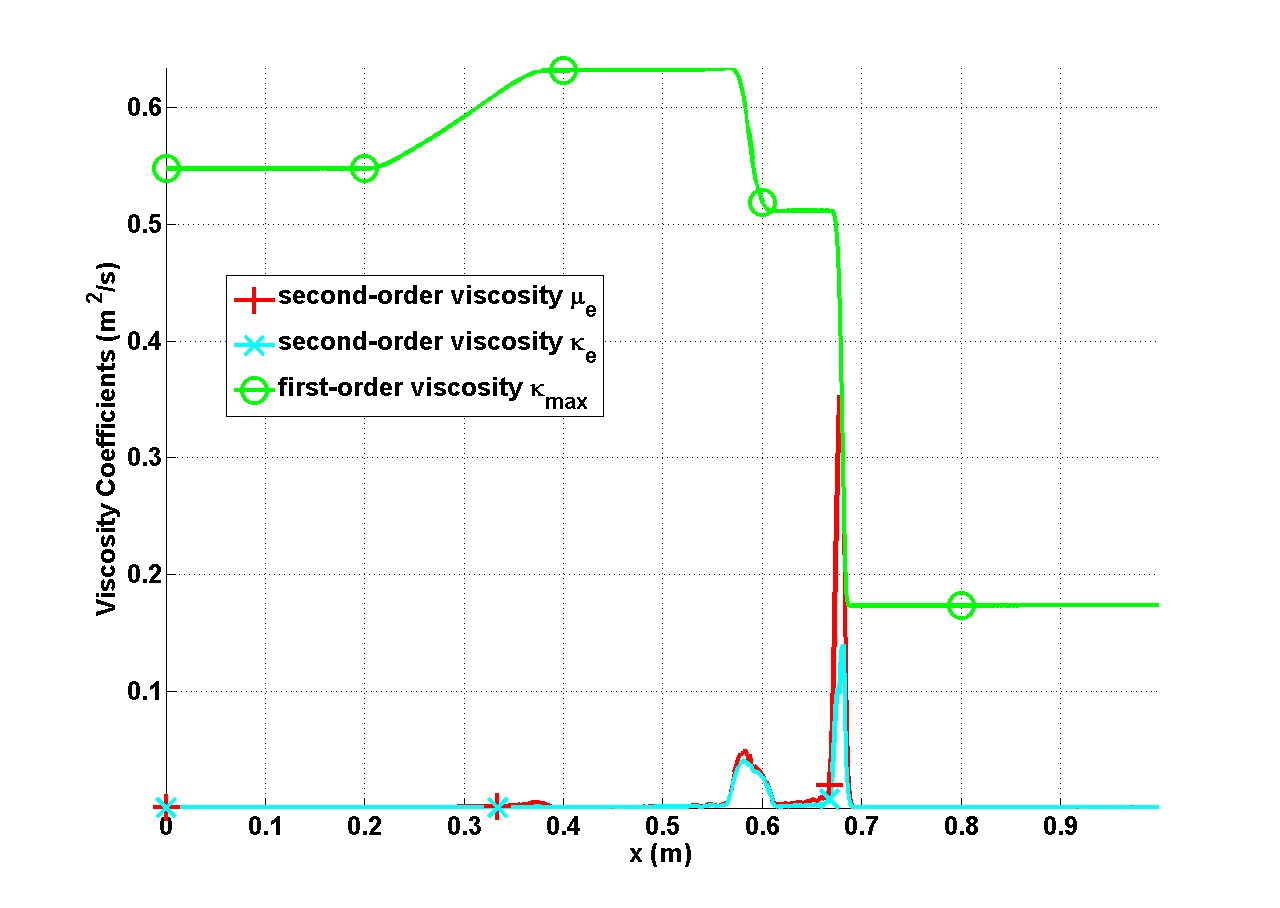
\includegraphics[width=0.495\textwidth]{plots/relaxation_two_phases_liquid_viscosity_kappa_mu.png}
                \caption{Viscosity coefficients for phase 1}
                \label{fig:viscosity_coeff_liq}
\end{figure}
\begin{figure}[H]								
%        \begin{subfigure}[b]{0.495\textwidth}
                \centering
                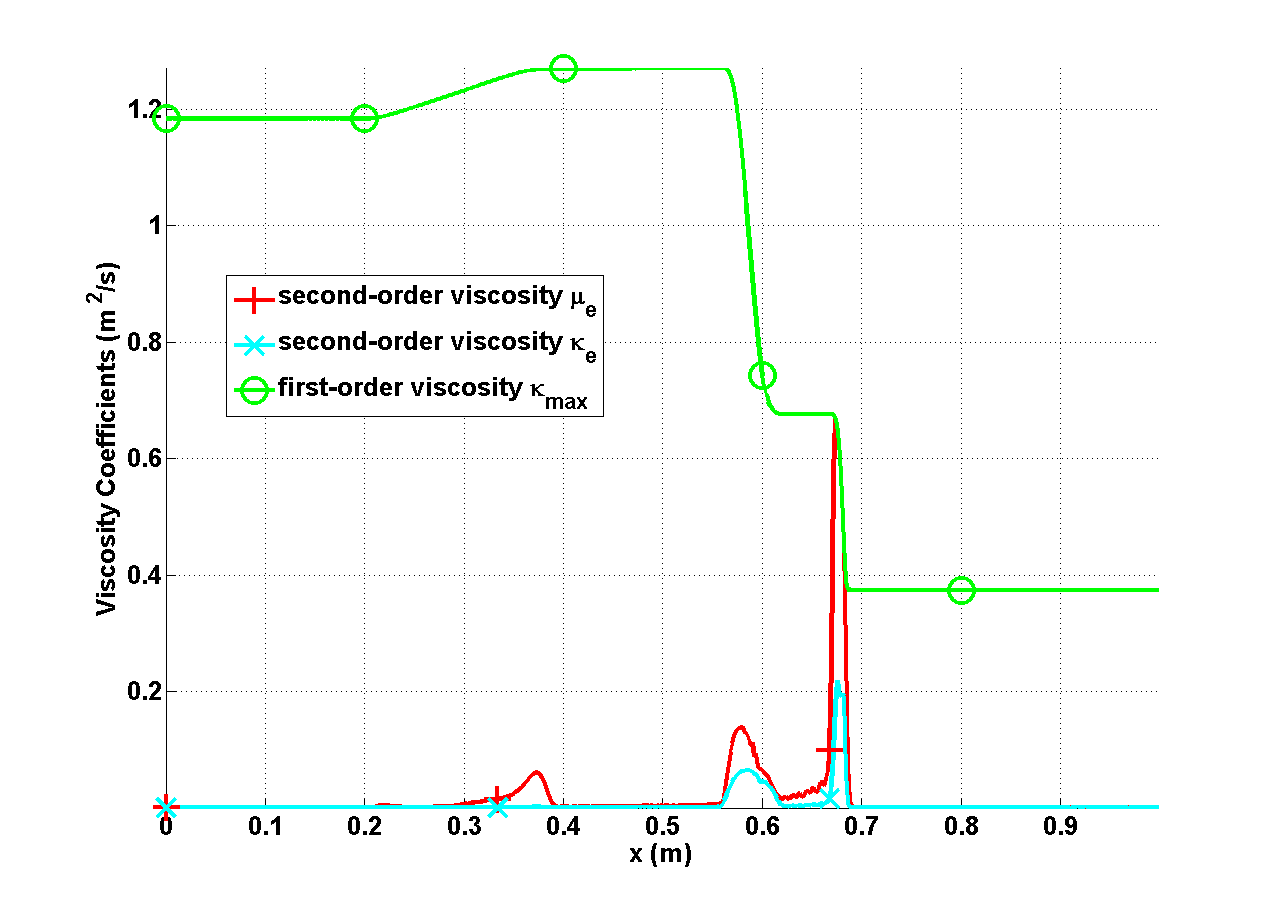
\includegraphics[width=0.495\textwidth]{plots/relaxation_two_phases_vapor_viscosity_kappa_mu.png}
                \caption{Viscosity coefficients for phase $2$}
                \label{fig:viscosity_coeff_vap}      
\end{figure}
\begin{figure}[H]				
        %\begin{subfigure}[b]{0.495\textwidth}
                \centering
                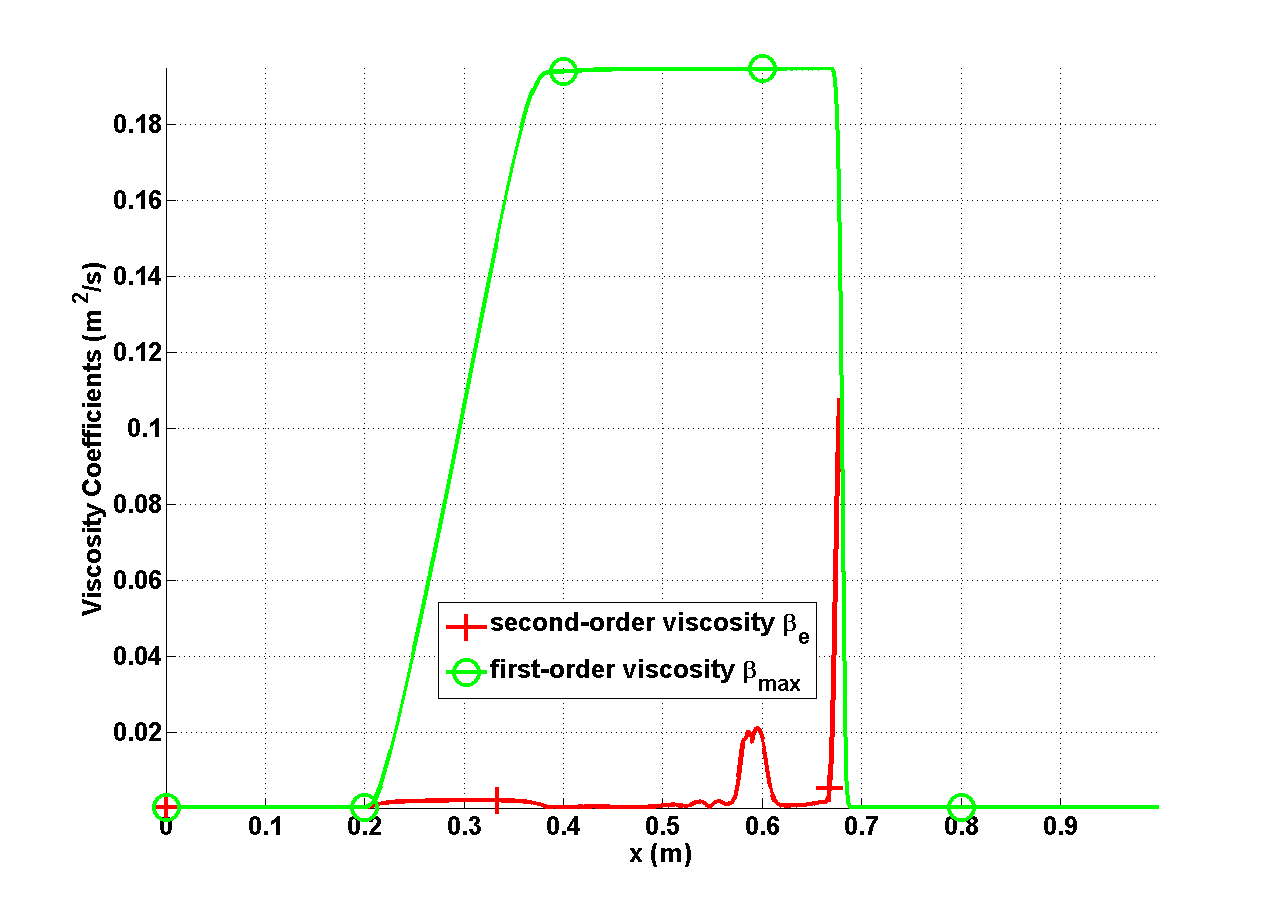
\includegraphics[width=0.495\textwidth]{plots/relaxation_two_phases_liquid_beta.png}
                \caption{Viscosity coefficients for the volume fraction.}
                \label{fig:viscosity_coeff_beta}
        %\end{subfigure}   
\end{figure}
%\begin{figure}[H]
%\centering
%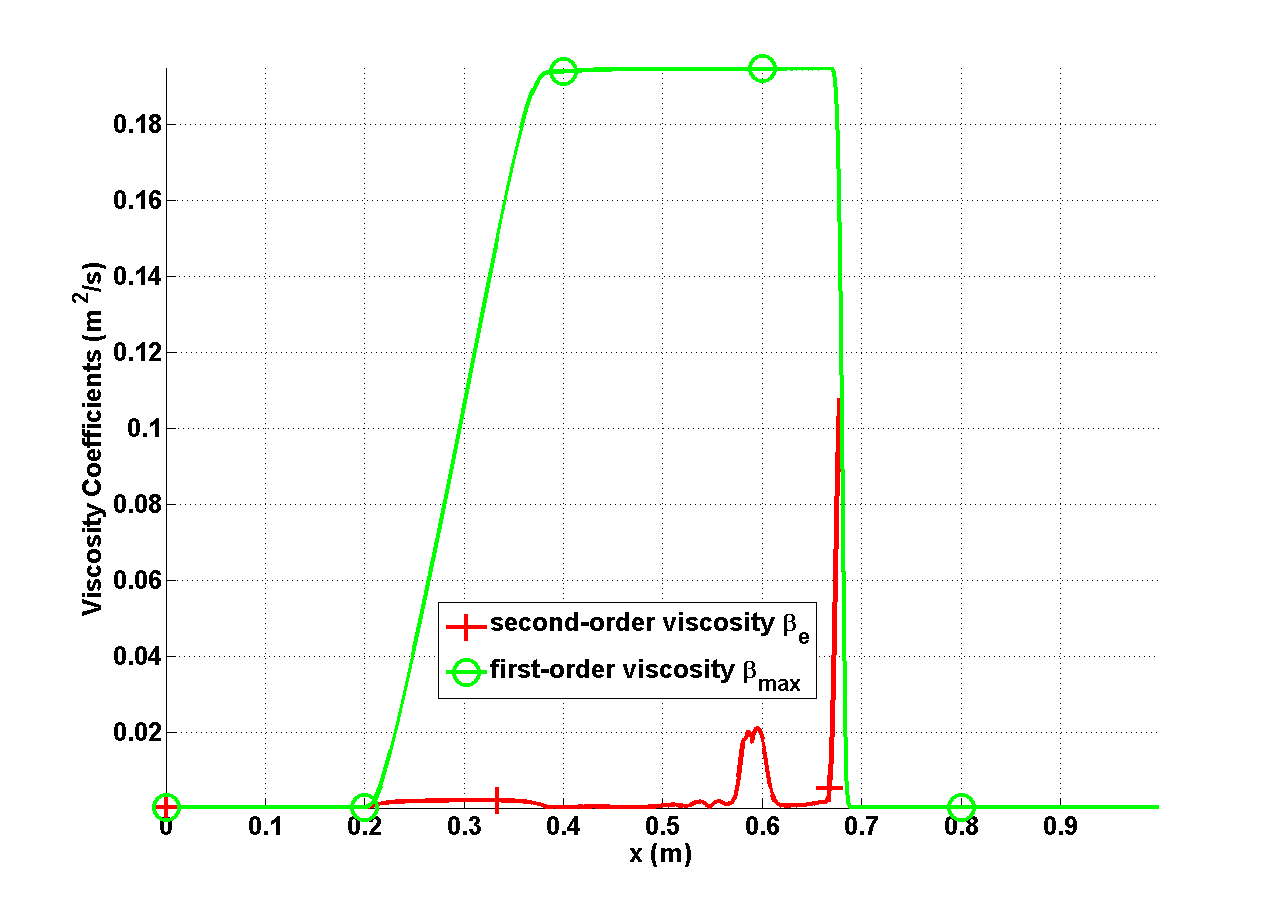
\includegraphics[width=0.495\textwidth]{plots/relaxation_two_phases_liquid_beta.png}
%\caption{Viscosity coefficients}
%\label{fig:viscosity_coeff_beta}
%\end{figure}        
%

%%%%%%%%%%%%%%%%%%%%%%%%%%%%%%%%%%%%%%%%%%%%%%%%%%%%%%%%%%%%%%%%%%%%%%%%%%%%%%%%
%\appendix
%\section{Appendix}

%%%%%%%%%%%%%%%%%%%%%%%%%%%%%%%%%%%%%%%%%%%%%%%%%%%%%%%%%%%%%%%%%%%%%%%%%%%%%%%%
%\section{Acknowledgments}
%This material is based upon work supported by the Department of Energy Rickover Fellowship Program in Nuclear Engineering.

%%%%%%%%%%%%%%%%%%%%%%%%%%%%%%%%%%%%%%%%%%%%%%%%%%%%%%%%%%%%%%%%%%%%%%%%%%%%%%%%
\bibliographystyle{ans}
\bibliography{bibliography}

\end{document}

